% !TEX root = ../my-thesis.tex
%
\chapter{Results}
\label{sec:results}

\section{Input resolution scaling}

Better understanding the impact of input resolution on the neural network training results is important for optimizing the network. The neural network was trained on inputs of varying resolution. The resolution of the inputs was scaled and the network parameters were scaled accordingly to the inputs, so larger resolution images also had more network parameters.

In table \ref{table:input} the input resolutions and the corresponding number of multiply–accumulate operations (MAC) are presented. MACs are a commonly used metric in machine learning because many of the tensor optimized accelerators compute $a \cdot x+b$ as a single operation \cite{nvidia_technical_blog_2022}, therefore one MAC is approximately 2 floating point operations (FLOPS).

\begin{table}
    \begin{tabular}{ |p{3cm}|p{3cm}|p{4cm}|  }
        \hline
        \multicolumn{3}{|c|}{Network input resolution, number of multiply–accumulate operations.} \\
        \hline
        x resolution & y resolution & MAC (G)                                                     \\
        \hline
        780          & 195          & 235.15                                                      \\
        520          & 130          & 104.39                                                      \\
        260          & 65           & 26.31                                                       \\
        156          & 39           & 9.49                                                        \\
        104          & 26           & 5.65                                                        \\
        52           & 13           & 1.09                                                        \\
        \hline
    \end{tabular}
    \caption{This table contains the input resolutions for 6 neural network architectures and their corresponding multiply–accumulate operations, which is a measure of the computational resources needed to train the network. To facilitate the larger input size the network adjusts the number of parameters, which results in an increase of computational resources to train.}
    \label{table:input}
\end{table}

When scaling the resolution to the labels used by the neural network there, it can been seen in figure \ref{fig:resolution-scaling} that higher resolution inputs do not necessarily result in better training results. In the case of the inception network that was tested, larger input resolutions also result in higher numbers of parameters and longer training times. The larger number of parameters could make it easier to overfit the network, especially with the limited size of the data set. However, when the resolution of the inputs is below 16900 pixels (260x65), the network is unable to resolve the features necessary to achieve an $rmse$ below $6 \cdot 10^{-3}$. If more training data was available, the network would be able to learn the features necessary to achieve a lower $rmse$ at the same resolution.

\begin{figure}[!htb]
    \centering
    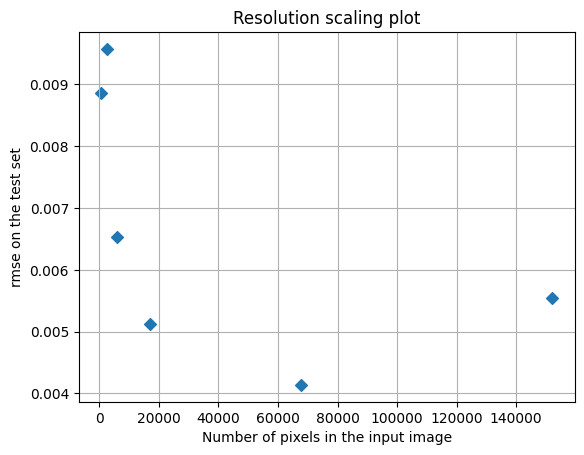
\includegraphics[width = \textwidth]{images/resolution-scaling.png}
    \caption{$rmse$ after training the neural network on the inputs at a given resolution over number of pixels in the input image. The pixel values are a product of the input image from the thermal camera height and width values after being scaled.} \label{fig:resolution-scaling}
\end{figure}

\section{Network Performance}

It is difficult to completely disentangle the increased network performance from the increased number of network parameters. However, it is not necessary to do so because ultimately the goal is to find a network that can be trained in a reasonable amount of time and that can be used to predict $\bar{\iota}$ values. The increased computational costs of training the network amounts to a few hours of training time on a single GPU. The network that was trained on the 520x130 input images was able to achieve this goal. The 520x130 network was able to achieve an $rmse$ of $4.13 \cdot 10^{-3}$ in 8 hours of training time on a single GPU, and the next best result was given by the 260x65 network with an $rmse$ of $5.12 \cdot 10^{-3}$ for a 50\% reduction in overall training time.

Figure \ref{fig:iota_vs_pred} shows the simulated $\bar{\iota}$ values vs the neural network reconstruction of $\bar{\iota}$ for the validation and test data sets for the two highest performance networks. As mentioned in section \ref{sec:data}, the neural network was trained on a data set that was split into training, validation, and test data sets but the distribution of $\bar{\iota}$ values was not uniform. This can be clearly seen in this graph, with the five independent programs worth of data being used for testing. The values for the test data set are normalized to mean zero and standard deviation one for the purposes of this plot but in the actual training the training data set was used to normalize the test data. The reconstructed $\iota$ values are then normalized to the test set. It can be seen in the right plot, the network slightly overestimates lower $\bar{\iota}$ values and slightly underestimates higher $\bar{\iota}$ values. The left plot, which shows the highest performance model does not show as much bias as the right plot, but the bias is still present. The bias is likely due to the limited size of the data set and the limited distribution of $\bar{\iota}$ values.


\begin{figure}[!htb]
    \centering
    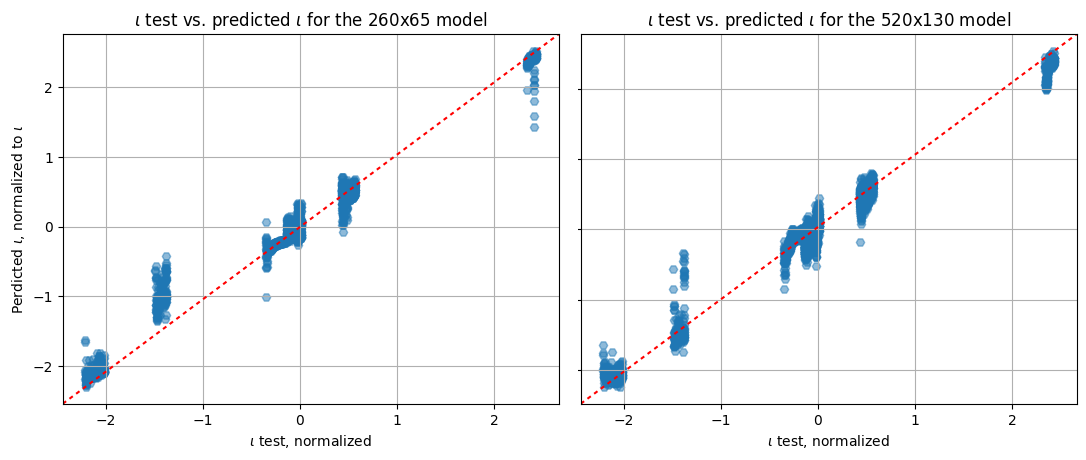
\includegraphics[width = \textwidth]{images/iota_vs_pred.png}
    \caption{$\bar{\iota}$ reconstruction with top two networks.} \label{fig:iota_vs_pred}
\end{figure}

We can see a similar trend in the violin plots in figure \ref{fig:kde}. In this plot the distribution of the L2 error kernel density estimate (KDE) is shown for all six networks. It should be noted that the KDE is not a probability distribution, but it is a good way to visualize the distribution of the error, and it is a good way to compare the error distributions of the different networks. The point-wise L2 error is defined as:

\begin{equation}
    \label{eq:l2}
    \text{L2 error} = (y_i - \hat{y}_i)^2
\end{equation}

where $y_i$ is the true value of $\bar{\iota}$ and $\hat{y}_i$ is the predicted value of $\bar{\iota}$. KDE is defined as:

\begin{equation}
    \label{eq:kde}
    \text{KDE} = \frac{1}{n} \sum_{i=1}^n \frac{1}{h} \sum_{j=1}^n K\left(\frac{y_i - y_j}{h}\right)
\end{equation}

where $n$ is the number of data points, $h$ is the bandwidth of the kernel, and $K$ is the kernel function. The bandwidth is chosen to be $0.1$ for all of the KDE plots. The kernel function used is the Gaussian kernel:

\begin{equation}
    \label{eq:gaussian}
    K(x) = \frac{1}{\sqrt{2 \pi}} e^{-\frac{x^2}{2}}
\end{equation}

Since values below zero are irrelevant to L2 error, the distributions are truncated at zero. The KDE is calculated for each network and then the KDE is normalized to the entire dataset. The KDE is then plotted as a violin plot, which is a box plot with the kernel density estimate plotted as a density function. The KDE is plotted as a density function because it is not a probability distribution. The two networks that exhibit best performance can be seen to have higher q-factors than the other networks.

\begin{figure}[!htb]
    \centering
    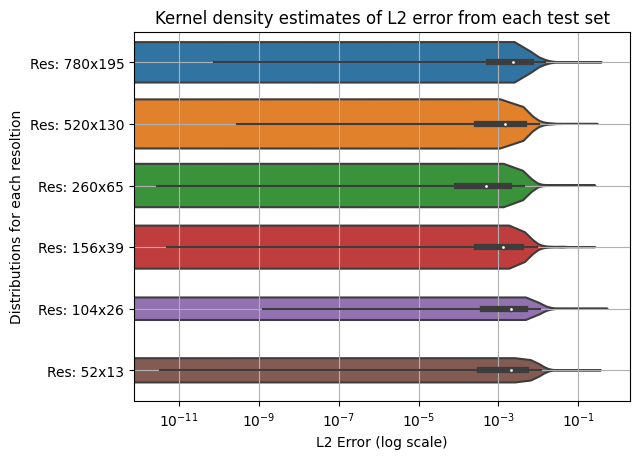
\includegraphics[width = \textwidth]{images/kde_plot.png}
    \caption{Kernel density estimate of L2 error from each trained neural network on the test datasets.} \label{fig:kde}
\end{figure}

